\documentclass[twoside,twocolumn]{article}
\usepackage{amsmath}
\usepackage{blindtext} % Package to generate dummy text throughout this template 
\usepackage{graphicx}
\usepackage{natbib}
\usepackage{lmodern}
\usepackage{color}
\usepackage{listings}
\lstdefinestyle{customc}{
  belowcaptionskip=1\baselineskip,
  breaklines=true,
  frame=l,
  xleftmargin=\parindent,
  language=C,
  showstringspaces=false,
  basicstyle=\footnotesize\ttfamily,
  keywordstyle=\bfseries\color{green!40!black},
  commentstyle=\itshape\color{purple!40!black},
  identifierstyle=\color{blue},
  stringstyle=\color{orange},
  xleftmargin=0.5cm
}


\usepackage[sc]{mathpazo} % Use the Palatino font
\usepackage[T1]{fontenc} % Use 8-bit encoding that has 256 glyphs
\linespread{1.05} % Line spacing - Palatino needs more space between lines
%\usepackage{microtype} % Slightly tweak font spacing for aesthetics

\usepackage[english]{babel} % Language hyphenation and typographical rules

\usepackage[hmarginratio=1:1,top=32mm,columnsep=20pt]{geometry} % Document margins
\usepackage[hang, small,labelfont=bf,up,textfont=it,up]{caption} % Custom captions under/above floats in tables or figures
\usepackage{booktabs} % Horizontal rules in tables

\usepackage{lettrine} % The lettrine is the first enlarged letter at the beginning of the text

\usepackage{enumitem} % Customized lists
\setlist[itemize]{noitemsep} % Make itemize lists more compact

\usepackage{abstract} % Allows abstract customization
\renewcommand{\abstractnamefont}{\normalfont\bfseries} % Set the "Abstract" text to bold
\renewcommand{\abstracttextfont}{\normalfont\small\itshape} % Set the abstract itself to small italic text

\usepackage{titlesec} % Allows customization of titles
\renewcommand\thesection{\Roman{section}} % Roman numerals for the sections
\renewcommand\thesubsection{\roman{subsection}}
\titleformat{\section}[block]{\large\scshape\centering}{\thesection.}{1em}{} % Change the look of the section titles
\titleformat{\subsection}[block]{\large}{\thesubsection.}{1em}{} % Change the look of the section titles

\usepackage{fancyhdr} % Headers and footers
\pagestyle{fancy} % All pages have headers and footers
\fancyhead{} % Blank out the default header
\fancyfoot{} % Blank out the default footer
\fancyhead[C]{FYS4150 $\bullet$ Project 3 $\bullet$ October 2016} % Custom header text
\fancyfoot[RO,LE]{\thepage} % Custom footer text

\usepackage{titling} % Customizing the title section

\usepackage{hyperref} % For hyperlinks in the PDF

%----------------------------------------------------------
%  COMMANDS
%---------------------------------------------------------

\newcommand{\nl}{
	
	\medskip
	\noindent
}
\newcommand{\SE}{Schroedinger equation }
\newcommand{\CI}{Coulomb interactions}
\newcommand{\sun}{\odot}
\newcommand{\planet}{\bullet}
\newcommand{\AU}{\text{AU}}
\newcommand{\Yr}{\text{Yr}}
\newcommand{\err}[1]{\mathcal{O}(#1)}
%--------------------------------------------



%----------------------------------------------------------------------------------------
%	TITLE SECTION
%----------------------------------------------------------------------------------------

\setlength{\droptitle}{-4\baselineskip} % Move the title up

\pretitle{\begin{center}\Huge\bfseries} % Article title formatting
	\posttitle{\end{center}} % Article title closing formatting
\title{FYS4150 - Project 3} % Article title
\author{%
	\textsc{Vegard R\o{}nning \& Heine H. Ness \& Sindre R. Bilden} \\[1ex] % Your name
	\normalsize University of Oslo \\ % Your institution
	\normalsize \href{mailto:vegard.ronning@fys.uio.no}{vegard.ronning@fys.uio.no}\ ; \href{mailto:h.h.ness@fys.uio.no}{h.h.ness@fys.uio.no}\ ; \href{mailto:s.r.bilden@fys.uio.no}{s.r.bilden@fys.uio.no}\\% Your email address
	\footnotesize \href{https://github.com/sindrerb/FYS4150-Collaboration/tree/master/Doc/Project3}{github.com/sindrerb/FYS4150-Collaboration/tree/master/Doc/Project3}
	%\and % Uncomment if 2 authors are required, duplicate these 4 lines if more
	%\textsc{Jane Smith}\thanks{Corresponding author} \\[1ex] % Second author's name
	%\normalsize University of Utah \\ % Second author's institution
	%\normalsize \href{mailto:jane@smith.com}{jane@smith.com} % Second author's email address
}
%----------------------------------------------------------------------------
\date{\today} % Leave empty to omit a date
\renewcommand{\maketitlehookd}{%
\begin{abstract}

\end{abstract}
}

%----------------------------------------------------------------------------

\begin{document}
	
% Print the title
\maketitle

%----------------------------------------------------------------------------
%	ARTICLE CONTENTS
%----------------------------------------------------------------------------
\section{Introduction}
\lettrine[nindent=0em,lines=2]{Q}uantum \blindtext
%----------------------------------------------------------------------------
\section{Methods}
\label{sec:methods}
\blindtext
\blindtext
%----------------------------------------------------------------------------
\newpage
\section{Implementation}
\label{sec:implementation}
Every planet in our solar system is affected by the gravitational force from the sun and other nearby planets. Where the gravitational force is
\begin{equation}
F_{G}=G\frac{M_\circ M_\planet}{r^2}
\end{equation} 
where $M_\circ$ and $M_\planet$ are the masses of two arbitrary objects. Decomposing the force into Cartesian coordinates, the components may be represented
\begin{equation*}
\hspace{-0.5cm}F_x=-\frac{GM_\circ M_\planet x}{r^3},F_y=-\frac{GM_\circ M_\planet y}{r^3},F_z=-\frac{GM_\circ M_\planet z}{r^3}
\end{equation*}
By Newton's second law the the relation between acceleration and position, we have the relation between the position of the planet and the total force component acting on the planet.
\begin{equation*}
\frac{d^2x}{dt^2}=\frac{F_x}{M_\planet},\hspace{0.6cm}\frac{d^2y}{dt^2}=\frac{F_y}{M_\planet},\hspace{0.6cm}\frac{d^2z}{dt^2}=\frac{F_z}{M_\planet}
\end{equation*}
Using the fact that Earth orbits the Sun in an almost circular motion \citep{NASA:orbit}, units of earth masses may be achieved by setting the centripetal force of the orbit equal to the gravitational force and solve for $GM_\sun$. Where $M_\sun$ is the mass of the Sun.
\begin{equation}
GM_\sun = 4\pi^2 \frac{\AU^3}{\Yr^2} \label{eq:units}
\end{equation}
Astronomical Units $\AU$ and years $\Yr$ are defined as the distance from Earth to the sun and the orbit time of Earth respectively. Equation \ref{eq:units} introduces Earth masses, Astronomical Units and Years as natural units for this system.\nl
In total the system gets three sets of coupled differential equations per object in the system, which has to be solved to describe the system properly.
\begin{align}
&\frac{dx}{dt}=v_x &\wedge \hspace{0.5cm} &\frac{dv_x}{dt}=\frac{F_x}{M_\planet}\label{eq:set_x}\\
&\frac{dy}{dt}=v_y &\wedge \hspace{0.5cm} &\frac{dv_y}{dt}=\frac{F_y}{M_\planet}\label{eq:set_y}\\
&\frac{dz}{dt}=v_v &\wedge \hspace{0.5cm} &\frac{dv_z}{dt}=\frac{F_z}{M_\planet}\label{eq:set_z}
\end{align}
The system may be described with numerical methods by discretizing equations (\ref{eq:set_x}-\ref{eq:set_z}). Letting  $t\rightarrow t_i=t_0+ih, i\in \mathbb{N}$, $x\rightarrow x_i$ and $v\rightarrow v_i$ be the new discretized relations with the initial conditions $x(t_0)=x_0$ and $v(t_0)=v_0$ where $x_0$ and $v_0$ is known, and $h=\frac{t_{max}-t_0}{N} $. The equations may be solved by Euler's method resulting in an algorithm with an error $\err{h^2}$ at each calculation. Here $a_{k,i}=\frac{F_k(k_i)}{M_\planet}$ where $k$ represents an axis label.
\begin{lstlisting}[style=customc]
x[i+1]=x[i]+h*xV[i]
y[i+1]=y[i]+h*yV[i]
z[i+1]=z[i]+h*zV[i]
xV[i+1]=xV[i]+h*xA[i]
yV[i+1]=yV[i]+h*yA[i]
zV[i+1]=zV[i]+h*zA[i]
\end{lstlisting}

Or with the more stable Verlet Vocity method reducing the error to $\err{h^3}$ for a calculation. 
\begin{lstlisting}[style=customc]
x[i+1]=x[i]+h*xV[i]+0.5*h*xA[i]
y[i+1]=y[i]+h*yV[i]+0.5*h*yA[i]
z[i+1]=z[i]+h*zV[i]+0.5*h*zA[i]
xV[i+1]=xV[i]+0.5*h*h*(xA[i+1]+xA[i])
yV[i+1]=yV[i]+0.5*h*h*(yA[i+1]+yA[i])
zV[i+1]=zV[i]+0.5*h*h*(zA[i+1]+zA[i])
\end{lstlisting}
These algorithms were implemented in a script that simulates the dynamics of the Sun and Earth. 

All code and results are found in the GitHub repository\nl
{\small \href{https://github.com/sindrerb/FYS4150-Collaboration/tree/master/Doc/Project3}{github.com/sindrerb/FYS4150-Collaboration/}}
\section{Results and discussion}
\label{sec:results}

	
	\begin{table}[h]
\caption{Table showing the three lowest computed eigenvalues $\lambda$ with $N$ mesh points, compared to the exact $\lambda_0=3$,$\lambda_1=7$ and $\lambda_2=11$.}\label{tbl:convergence}
		\centering
		\begin{tabular}{|l|l|l|l|}\hline
			$N$ & $\lambda_0$ & $\lambda_1$ & $\lambda_2$\\ \hline
			10 & 2.68672 & 6.11302 & 11.0574\\
			50 & 2.98745 & 6.93692 & 10.8453\\
			100& 2.99687 & 6.98432 & 10.9617\\
			200& 2.99916 & 6.99610 & 10.9904\\
			300& 2.99961 & 6.99828 & 10.9958\\
			400& 2.99986 & 6.99903 & 10.9976\\
			500& 2.99993 & 6.99937 & 10.9986\\\hline
\end{tabular}
\end{table}
\begin{figure}[p]
%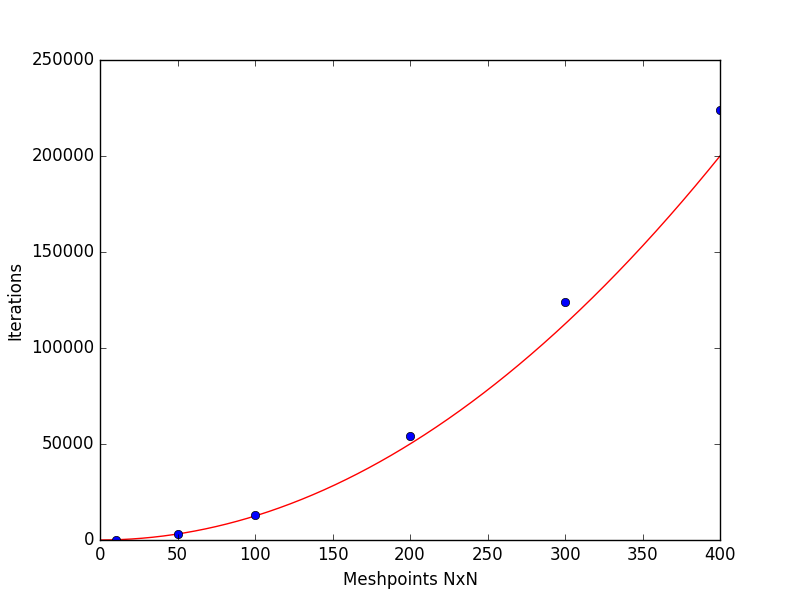
\includegraphics[width=0.5\textwidth]{figures/iterations.png} 
		\caption{Graph over the number of iterations for a given set of mesh points $N$. The solid red line is proportional to $N^2$ as a comparison.}\label{fig:iterations}
\end{figure}

%----------------------------------------------------------------------------
\section{Summary and Conclusion}
\label{sec:conclusion}
%----------------------------------------------------------------------------
	%\twocolumn[]
	
\end{document}
